\documentclass[a4paper,10pt]{article}
\usepackage[ngerman]{babel}		%dt. Übersetzung und Umlaute
\usepackage[utf8]{inputenc}		%Umlaute direkt eingeben
\usepackage{mathtools}			%Mathekrams
\usepackage{paralist}			%bessere Listen
\usepackage{amssymb}			%Mathesymbole
\usepackage{amsthm}			%typesetting theorems (Text über = u.ä.)
\usepackage{fancyhdr} 			%Headerstyles
\usepackage{verbatim}			%Sourcecode einfügen
\usepackage[margin=2.0cm,headheight=40pt,top=3cm]{geometry}
\usepackage{tikz}
\usepackage{cancel}
\usepackage{stmaryrd}
\usepackage{colortbl}
\usepackage{tabularx}
\usepackage{stmaryrd} %Package für den coolen Blitz
\newcolumntype{L}[1]{>{\raggedright\arraybackslash}p{#1}} % linksbündig mit Breitenangabe
\usetikzlibrary{matrix,positioning,arrows, automata}

\pagestyle{fancy}
\renewcommand{\headrulewidth}{0.4pt}
\renewcommand{\footrulewidth}{0.4pt}
\lhead{Blatt 06}
\rhead{}
\cfoot{}
\rfoot{\thepage}
\begin{document}
	\parindent0pt
	\textbf{Aufgabe 01}
	\begin{compactenum} [(a)]
		\item
		\begin{compactenum} [(i)]
			\item $ R_r := R \cup \{(a,a),(b,b),(c,c),(d,d)\} $
			\item Es ist nicht möglich durch hinzufügen von Paaren $ (x,y) \in A \times A $ die Relation $ R $ so zu erweitern, dass die Erweiterung $ R_a $ antisymmetrisch ist, da $ R $ bereits nicht antisymmetrisch ist: $ (a,d) $ und $ (d,a) \in R $ und $ a \neq d \Rightarrow $ R ist nicht antisymmetrisch.
			\item $ R_k := R \cup \{(a,c),(a,e),(b,e),(c,e),(d,e)\} $
		\end{compactenum}
		\item $ R_1 $ hat folgende Eigenschaften:
		\begin{compactitem}
			\item Nicht reflexiv: $ (-4,-4) \not\in R_1 $
			\item Symmetrisch: Wenn $ (x,y) \in R_1 $ und somit $ x\cdot y \leq 3 $ dann ist auch $ y\cdot x \leq 3 $ und somit $ (y,x) \in R_1 $
			\item Nicht antisymmetrisch: weil symmetrisch
			\item Nicht konnex: $ (-4,-3) \not\in R_1 $ und $ (-3,-4) \not\in R_1 $
			\item Nicht transitiv: $ (-4,0) \in R_1 $ und $ (0,-3) \in R_1 $ aber $ (-4,-3) \not\in R_1 $
		\end{compactitem}
		$ R_2 $ hat folgende Eigenschaften:
		\begin{compactitem}
			\item Reflexiv: für jede Menge $ a \in M_2 $ gilt: $ a \cap a = a \neq \emptyset $
			\item Symmetrisch: Für jede Menge $ a,b \in M_2 $ gilt: Wenn $ a\cap b \neq \emptyset $ dann ist auch $ b\cap a \neq \emptyset $
			\item Nicht antisymmetrisch: weil symmetrisch
			\item Nicht konnex: $ (\{1\},\{2\}) \not\in R_2 $ und $ (\{2\},\{1\}) \not\in R_2 $
			\item Nicht transitiv: $ (\{1\}, \{1,2\}) \in R_2 $ und $ (\{1,2\},\{2\}) \in R_2 $ aber $ (\{1\},\{2\}) \not\in R_2 $
		\end{compactitem}
	\end{compactenum} \
	
	\textbf{Aufgabe 02}\\
	\begin{compactitem}
		\item $ t_1 := f(v_1,f(v_0,v_2)) $\\
		
		$ \llbracket t_1\rrbracket^\mathcal{I} =  f$(Spock, $f$(Stein,Schere)) = $f$(Spock,Stein) = Spock \\
		
		\item $ t_2 := f(f(f(v_0,v_0),c),f(v_3,f(v_4,v_5))) $\\
		\begin{tabbing}
			$ \llbracket t_2\rrbracket^\mathcal{I}$
			\= $ = f(f(f($Stein,Stein$),$Spock$),f($Papier$, f($Papier,Papier$)))$ \\
			\> $= f(f($Stein,Spock$),$Papier$) = f($Spock,Papier$) = $ Papier 
		\end{tabbing}
	\end{compactitem} \
		
	\textbf{Aufgabe 03}\\
	\begin{compactenum} [(a)]
		\item $ \sigma $-Term, atomare $ \sigma $-Formel und/oder FO[$ \sigma $]-Formel \\
		
		\begin{tabular}  {c|L{4cm}|L{5cm}|L{5cm}}
			&$ \sigma $- Term & atomare $ \sigma $-Formel & FO[$ \sigma $]-Formel\\ \hline
			(i) & kein $ \sigma $-Term, da das '$ \vee $'$ \not\in A_{\sigma -Terme}$ & keine atomare $ \sigma $-Formel, da diese kein '$ \vee $' beinhalten darf & keine FO[$ \sigma $]-Formel, da nur die Veroderung zweier FO[$ \sigma $]-Formeln wieder eine FO[$ \sigma $]-Formel ergibt. Hier handelt es sich um die Veroderung von zwei $ \sigma $-Termen \\ \hline
			(ii) & kein $ \sigma $-Term, da $ R \not\in A_{\sigma -Terme}$ & atomare $ \sigma $-Formel & FO[$ \sigma $]-Formel \\ \hline
			(iii) & kein $ \sigma $-Term, da u.a. $ R \not\in A_{\sigma -Terme}$ & keine atomare $ \sigma $-Formel, da diese kein '$ \vee $' beinhalten darf & keine FO[$ \sigma $]-Formel, da die Veroderung von einem $ \sigma $-Term mit einer FO[$ \sigma $]-Formel keine FO[$ \sigma $]-Formel ergibt \\ \hline
			(iv) & kein $ \sigma $-Term, da u.a. $ R \not\in A_{\sigma -Terme}$ & keine atomare $ \sigma $-Formel, da diese u.a. kein '$ \wedge $' beinhalten darf & keine FO[$ \sigma $]-Formel, da genau genommen der '$ \leftrightarrow $'-Pfeil nicht zu den rekursiven Regeln der FO[$ \sigma $]-Formel Definition gehört 
		\end{tabular} \\
		\newpage
		\item \begin{compactitem}
			\item $ \mathcal{A} \not\cong \mathcal{B} $. Begründung: Angenommen es ex. ein Isomorphismus $ \pi : \mathcal{A} \rightarrow \mathcal{B} $, dann folgt: \\
			\begin{compactitem}
				\item $ 2 = c^\mathcal{A} \rightarrow \pi(c^\mathcal{A}) = c^\mathcal{B} = w$\\
				$ \Rightarrow \pi(2) = w $
				\item $ (2,2,4) \in S^\mathcal{A} \rightarrow \pi(S^\mathcal{A}) = S^\mathcal{B} \ni (w,w,y)$ \\
				$ \Rightarrow \pi(4) = y $
				\item $ f^\mathcal{A}(4) = 5 \rightarrow \pi(f^\mathcal{A}(4)) = f^\mathcal{B}(y) = x $ \\
				$ \Rightarrow \pi(5) = x $
				\item $ f^\mathcal{A}(5) = 4 \rightarrow \pi(f^\mathcal{A}(5)) = f^\mathcal{B}(x) = z $ \\
				$ \Rightarrow \pi(4) = z $\\
				$ \Longrightarrow \lightning$ Widerspruch zu $ \pi(4) = y $
				
			\end{compactitem}
			\item Es gilt $ \mathcal{A} \cong \mathcal{C}$ mit der Abbildung $ \pi : \mathcal{A} \rightarrow \mathcal{C} $\\
			\begin{tabular} {c|c|c|c|c|c}
				A & 1 & 2 & 3 & 4 & 5 \\ \hline
				$ \pi(A) $ & c & d & e & b & a
			\end{tabular}
		\end{compactitem}
	\end{compactenum}\ \\ \\
		\textbf{Aufgabe 03}\\
		\begin{compactenum} [(a)]
			\item \ \\ 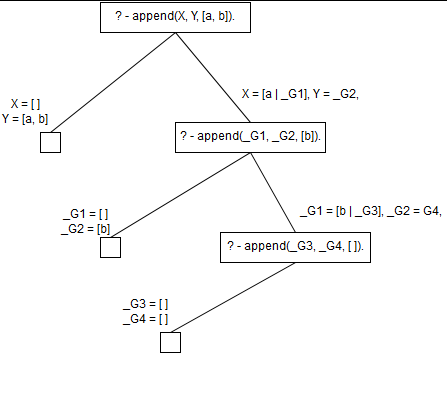
\includegraphics[width=4.5cm]{Blatt06_4a}\\
			\item 
			\begin{verbatim}
				tree(leaf(_)).
				tree(node(L, R)) :- tree(L), tree(R).	
			\end{verbatim} \ \\
			\item 
			\begin{verbatim}
				Inhalt..label(leaf(X), X).
				label(node(L, _), X) :- label(L,X).
				label(node(_, R), X) :- label(R,X).
			\end{verbatim} \\
			\item 
			\begin{verbatim}
				verkettet([], X, X).
				verkettet([H|T], X, [H|Y]) :-
				verkettet(T, X, Y).
				
				append([], Y, Y).
				append([H|T], Y, [H|T2]) :- verkettet(T, Y, T2).
			
				labels(leaf(X), [X]).
				labels(node(L, R), X) :-
				labels(L, X1),
				labels(R, X2),
				verkettet(X1, X2, X).
			\end{verbatim}
			
		\end{compactenum}
\end{document}
